\section{DL\_POLY Parallelisation}


\D{} is a distributed parallel molecular dynamics package based on
the Replicated Data parallelisation strategy 
\cite{smith-91a,smith-93a}.  In this section we briefly outline the basic
methodology. Users wishing to add new features \D{} will need to
be familiar with the underlying techniques as they are described (in
greater detail) in references \cite{smith-93b,smith-93a}).

\subsection{The Replicated Data Strategy}
\label{parallelisation}
The Replicated Data (RD) strategy \cite{smith-91a} is one of several
ways to achieve parallelisation\index{parallelisation} in MD. 
Its name derives from the
replication of the configuration data on each node of a parallel
computer (i.e. the arrays defining the atomic coordinates
$\vek{r}_{i}$, velocities $\vek{v}_{i}$ and forces $\vek{f}_{i}$, for
all $N$ atoms $\{i: i=1,\dots,N\}$ in the simulated system, are
reproduced on every processing node). In this strategy most of the
forces computation and integration of the equations of motion can be
shared easily and equally between nodes and to a large extent be
processed independently on each node. The method is relatively simple
to program and is reasonably efficient. Moreover, it can be
``collapsed'' to run on a single processor very easily.  However the
strategy can be expensive in memory and have high communication
overheads, but overall it has proven to be successful over a wide
range of applications.  These issues are explored in more detail in
\cite{smith-91a,smith-93a}.

Systems containing complex molecules present several difficulties.
They often contain ionic species, which usually require Ewald summation\index{Ewald!summation} methods \cite{allen-89a,smith-92b}, and {\em intra}-molecular
interactions in addition to {\em inter}-molecular forces.  These are
handled easily in the RD strategy, though the SHAKE\index{algorithm!SHAKE} algorithm
\cite{ryckaert-77a} requires significant modification \cite{smith-93b}.

The RD strategy is applied to complex molecular systems as follows:
\begin{enumerate}
\item Using the known atomic coordinates $\vek{r}_{i}$, each node
calculates
a subset of the forces acting between the atoms. These are usually
comprised of:
\begin{enumerate}
\item atom-atom pair forces (e.g. Lennard Jones, Coulombic etc.);
\item non-rigid atom-atom bonds;
\item valence angle\index{potential!valence angle} forces;
\item dihedral angle\index{potential!dihedral} forces;
\item improper dihedral angle\index{potential!improper dihedral} forces.
\end{enumerate}
\item The computed forces are accumulated in (incomplete) atomic 
force arrays $\vek{f}_{i}$ independently on each node;
\item The atomic force arrays are summed globally over all nodes;
\item The complete force arrays are used to update the atomic
velocities and positions.
\end{enumerate}
It is important to note that load balancing (i.e. equal and concurrent
use of all processors) is an essential requirement of the overall
algorithm. In \D{} this is accomplished for the pair forces with an
adaptation of the Brode-Ahlrichs\index{algorithm!Brode-Ahlrichs} scheme \cite{brode-86a}.


\subsection{Distributing the Intramolecular Bonded Terms}

\D{} handles the intramolecular\index{parallelisation!intramolecular terms}
in which the atoms involved in any given bond term are explicitly
listed. Distribution of the forces calculations is accomplished by the
following scheme:
\begin{enumerate}
\item Every atom in the simulated system is assigned a unique index
number from $1$ to $N$; 
\item Every intramolecular\index{parallelisation!intramolecular terms} bonded term $U_{type}$ in the system has a 
unique index number $i_{type}$: from $1$ to $N_{type}$ where $type$
represents a bond\index{potential!bond}, angle or dihedral\index{potential!dihedral}.
\item A pointer array $key_{type}(n_{type},i_{type})$ carries the 
indices of the specific atoms involved in the potential term labelled
$i_{type}$. The dimension $n_{type}$ will be $2,~3$ or $4$, if the
term represents a bond, angle or dihedral.
\item The array $key_{type}(n_{type},i_{type})$ is used to identify
the atoms in a bonded term and the appropriate form of interaction and
thus to calculate the energy and forces.  Each processor is assigned
the independent task of evaluating a block of
($Int(N_{total}/N_{nodes})$) interactions.
\end{enumerate}

The same scheme works for all types of bonded interactions.  The
global summation of the force arrays does not occur until all the
force contributions, including nonbonded forces has been completed.

\subsection{Distributing the Nonbonded Terms}

In \D{} the nonbonded\index{potential!nonbonded} interactions are handled with a Verlet neighbour
list\index{Verlet neighbour list} \cite{allen-89a} which is reconstructed at intervals during the
simulation. This list records the indices of all `secondary' atoms
within a certain radius of each `primary' atom; the radius being the
cut-off radius ($r_{cut}$) normally applied to the nonbonded\index{potential!nonbonded} potential
function, plus an additional increment ($\Delta r_{cut}$). The larger
radius ($r_{cut}+\Delta r_{cut}$) permits the same list to be used for
several timesteps\index{algorithm!multiple timestep} without requiring an update.  The frequency at which
the list must be updated clearly depends on the thickness of the
region $\Delta r_{cut}$.  In RD, the neighbour list\index{Verlet neighbour list} is constructed
{\em simultaneously} on each node and in such a way as to share the
total burden of the work equally between nodes. Each node is
responsible for a unique set of nonbonded interactions and the
neighbour list is therefore different on each node. \D{} uses a method
based on the Brode-Ahlrichs\index{algorithm!Brode-Ahlrichs} scheme 
\cite{brode-86a} (see figure \ref{BAscheme})
to construct the neighbour list. 

Additional modifications are necessary to handle the excluded atoms
\cite{smith-93a}. A distributed {\em excluded atoms
list} is constructed by \D{} at the start of the simulation. The list is
constructed so that the excluded atoms are referenced in the same
order as they would appear in the Verlet neighbour list if the bonded
interactions were ignored, allowing for the distributed structure of
the neighbour list.

~

\vskip 5mm
\begin{figure}[ht]
\begin{center}
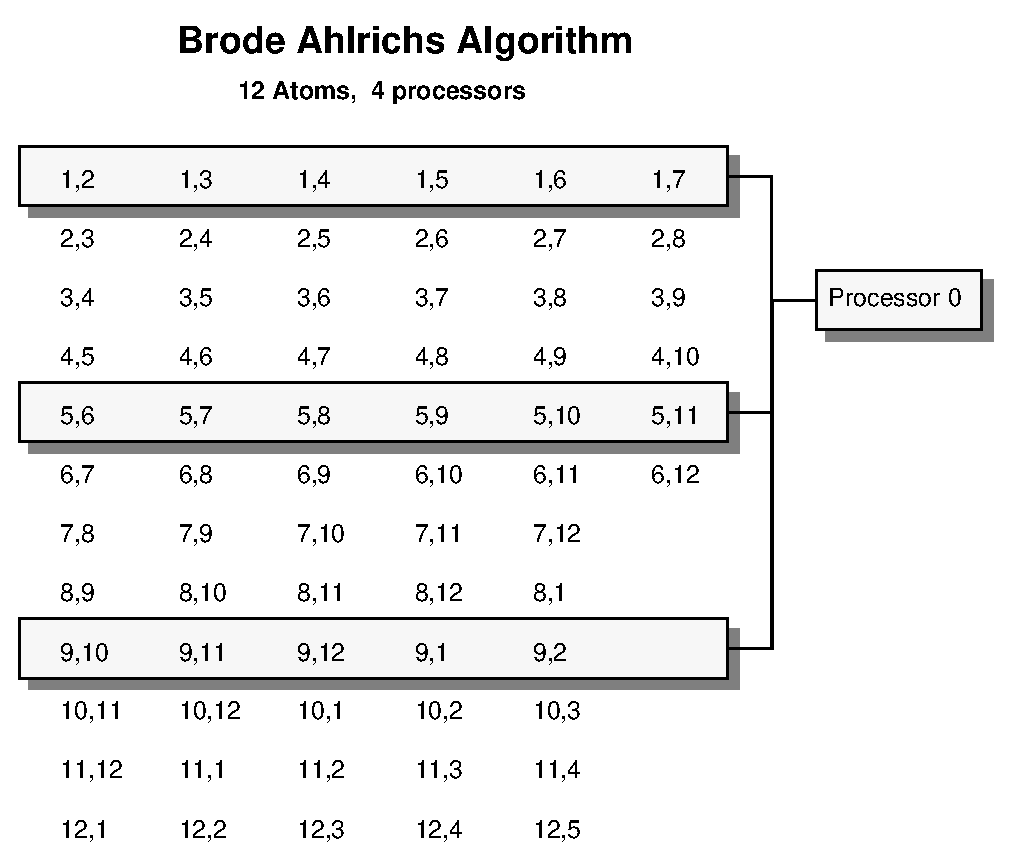
\includegraphics[height=12cm]{brode.eps}
\caption{The parallel implementation of the Brode-Ahlrichs algorithm.\label{BAscheme}}
\end{center}
This diagram illustrates the reordering of the upper triangular matrix
of n(n-1)/2 pair interactions so that the rows of the matrix are of
approximately equally length.  Each entry in the table consists of a
primary atom index (constant within a row) and a ``neighbouring'' atom
index.  Rows are assigned sequentially to nodes. In the diagram node 0
deals with rows 1, 5 and 9, node 1 to rows 2, 6, and 10 etc.
\end{figure}
\vskip 5mm

When a charge group scheme (as opposed to an atomistic scheme) is used
for the non-bonded terms, the group-group interactions are distributed
using the Brode-Ahlrichs\index{algorithm!Brode-Ahlrichs} approach. This makes the Verlet list\index{Verlet neighbour list}
considerably smaller, thus saving memory, but also results in a more
``coarse grain'' parallelism\index{parallelisation!Verlet neighbour list}. The consequence of which is that
performance with a large number of processors will degrade more
quickly than with the atomistic scheme.

Once the neighbour list has been constructed, each node of the
parallel computer may proceed independently to calculate the pair
force contributions to the atomic forces. 

\subsection{Modifications for the Ewald Sum}

For systems with periodic boundary conditions \D{} employs the Ewald Sum\index{Ewald!summation}
to calculate the Coulombic interactions (see section \ref{ewaldsum}).

Calculation of the real space component in \D{} employs the algorithm
for the calculation of the nonbonded interactions outlined above. The
reciprocal space component is calculated using the schemes described
in \cite{smith-92b}, in which the calculation can be
parallelised\index{parallelisation!Ewald summation} by
distribution of either $\vek{k}$ vectors or atomic sites. Distribution
over atomic sites requires the use of a global summation of the
$q_{i}\exp(-i\vek{k}\cdot\vek{r}_{j})$ terms, but is more efficient in
memory usage. Both strategies are computationally straightforward.
Subroutine {\sc ewald1} distributes over atomic sites and is often the
more efficient of the two approaches. Subroutine {\sc ewald1a}
distributes over the $\vek{k}$ vectors and may be more efficient on
machines with large communication latencies.

Other routines required to calculate the ewald sum include {\sc
ewald2}, {\sc ewald3} and {\sc ewald4}. The first of these calculates
the real space contribution, the second the self interaction
corrections, and the third is required for the multiple timestep
option.

\subsection{Modifications for SPME}

The SPME\index{Ewald!SPME} method requires
relatively little modification for parallel computing. The real space
terms are calculated exactly as they are for the normal Ewald sum, as
described above. The reciprocal space sum requires a 3D Fast Fourier
Transform (FFT), which in principle should be distributed over the
processors, but in \D{} the decision was made to implement a complete 3D
FFT on every processor. This is expensive in memory, and potentially
expensive in computer time. However a multi-processor FFT requires
communication between processors and this has significant impact on
the famed efficiency of the FFT. It transpires that a single processor
FFT is so efficient that the adopted strategy is still effective. The
charge array that is central to the SPME method (see section
\ref{spmesum}) is however built in a distributed manner and then
globally summed prior to the FFT operation.

\subsection{Three and Four Body Forces}

\D{} can calculate three/four body interactions of the valence\index{potential!valence angle}
angle type \cite{vessal-90a}. These are not dealt with in the same way
as the normal nonbonded\index{potential!nonbonded} interactions. They are generally very short
ranged and are most effectively calculated using a link-cell scheme
\cite{hockney-81a}. No reference is made to the Verlet neighbour list\index{Verlet neighbour list}
nor the excluded atoms list. It follows that atoms involved in the
same three/four-body\index{potential!three-body}\index{potential!four-body} term can interact via nonbonded (pair) forces and
ionic forces also. The calculation of the three/four-body terms is
distributed over processors on the basis of the identity of the
central atom in the bond. A global summation is required to specify
the atomic forces fully.

\subsection{Metal Potentials}

The simulation of metals by \D{} makes use of density dependent
potentials of the Sutton-Chen type \cite{sutton-90a}. The dependence on
the atomic density presents no difficulty however, as this class of
potentials can be resolved into pair contributions. This permits the
use of the distributed Verlet neighbour list\index{Verlet neighbour list} outlined above.

\subsection{Summing the Atomic Forces}

The final stage in the RD strategy, is the global summation of the
atomic force arrays. This must be done After all the contributions to
the atomic forces have been calculated. To do this \D{} employs a
global summation algorithm \cite{smith-91a}, which is generally a
system specific utility.

Similarly, the total configuration energy and virial must be obtained as
a global sum of the contributing terms calculated on all nodes.


\subsection{The SHAKE, RATTLE and Parallel QSHAKE Algorithms}
\label{parshake}

The SHAKE\index{algorithm!SHAKE} and RATTLE\index{algorithm!RATTLE}
algorithms are methods for constraining rigid bonds. Parallel
adaptations of both are couched in the Replicated
Data strategy. The essentials of the methods are as follows.

\begin{enumerate}
\item The  bond constraints acting in the simulated system are shared
equally between the processing nodes.
\item Each node makes a list recording which atoms are bonded by 
constraints\index{constraints!bond} it is to process. Entries are zero if the atom is not
bonded.
\item A copy of the array is passed to each other node in turn. 
The receiving node compares the incoming list with its own and keeps a
record of the shared atoms and the nodes which share them.
\item In the first stage of the SHAKE\index{algorithm!SHAKE} algorithm, the atoms are
updated through the usual Verlet\index{algorithm!Verlet} algorithm, without regard to the bond
constraints\index{constraints!bond}.
\item In the second (iterative) stage of SHAKE\index{algorithm!SHAKE}, each node calculates
the incremental correction vectors for the bonded\index{potential!bond} atoms in its own list
of bond constraints. It then sends specific correction vectors to all
neighbours that share the same atoms, using the information compiled
in step 3.
\item When all necessary  correction vectors have been received and
added
the positions of the constrained atoms are corrected.
\item Steps 5 and 6 are repeated until the bond constraints are
converged.
\item After convergence the coordinate arrays on each node are 
passed to all the other nodes. The coordinates of atoms that are {\em
not} in the constraint list of a given node are taken from the
incoming
arrays (an operation we term {\em splicing}).
\item Finally, the change in the atom positions is used to calculate
the
atomic velocities.
\end{enumerate}

The above scheme is complete for a implementation based on the
leapfrog integration algorithm. However a velocity Verlet (VV) scheme
requires additional steps.

\begin{enumerate}
\item Step 9 above does not apply for VV. The velocity is integrated
under the normal VV scheme.
\item When the velocity is updated, iteration of the constraint force
takes place. The incremental changes to the velocity are communicated
between nodes sharing constrained atoms as for the bondlength
constraints.
\item Iteration is repeated until the bond constraints are
converged.
\item After convergence the velocity arrays on each node are 
passed to all the other nodes by {\em splicing}.
\end{enumerate}

This scheme contains a number of non-trivial operations, which are
described in detail in \cite{smith-93b}. However some general comments
are worth making.

The compilation of the list of constrained atoms on each node, and the
circulation of the list (items 1 - 3 above) need only be done once in
any given simulation. It also transpires that in sharing bond
contraints\index{constraints!bond} between nodes, there is an advantage to keeping as many of
the constraints pertaining to a particular molecule together on one
node as is possible within the requirement for load balancing. This
reduces the data that need to be transferred between nodes during the
iteration cycle. It is also advantageous, if the molecules are small,
to adjust the load balancing between processors to prevent shared
atoms. The loss of balance is compensated by the elimination of
communications during the SHAKE\index{algorithm!SHAKE} cycle. These 
techniques are exploited by \D{}.

The QSHAKE\index{algorithm!QSHAKE} algorithm is an extension of the SHAKE algorithm for 
constraint bonds\index{constraints!bond} between rigid bodies\index{rigid body}. The parallel strategy is 
very similar to that of SHAKE\index{algorithm!SHAKE}. The only significant difference is that increments
to the atomic forces, not the atomic positions, are passed between
processors at the end of each iteration.
